\documentclass[12pt]{article}
\usepackage{natbib}
\usepackage[french]{babel}
\usepackage[T1]{fontenc}
\usepackage{url}
\usepackage[utf8x]{inputenc}
\usepackage{amsmath}
\usepackage{mathtools}
\usepackage{graphicx}
\graphicspath{{images/}}
\usepackage{parskip}
\usepackage{amssymb}
\usepackage{xurl}
\usepackage{caption}
\usepackage{geometry}
\usepackage{float}
\usepackage[shortlabels]{enumitem}
\geometry{hmargin = 2.5cm, vmargin = 2.5cm}

\title{Classification Algorithms}							% Title
\date{\today}											% Date

\makeatletter
\let\thetitle\@title
\let\theauthor\@author
\let\thedate\@date
\makeatother

\begin{document}
%%%%%%%%%%%%%%%%%%%%%%%%%%%%%%%%%%%%%%%%%%%%%%%%%%%%%%%%%%%%%%%%%%%%%%%%%%%%%%%%%%%%%%%%%

\begin{titlepage}
	\centering
    
\includegraphics[scale = 0.7]{img/University.png}\\[1.0 cm]	% University Logo
    \textsc{\LARGE \newline\newline Faculté des Sciences appliquées}\\	% University Name
	\textsc{\Large  ELEN062-1: Introduction to Machine Learning}\\[0.5 cm]	% Course Code
	\rule{\linewidth}{0.2 mm} \\[0.4 cm]
	{\huge \bfseries \thetitle}
	\rule{\linewidth}{0.2 mm} \\[2 cm]
	
	\begin{minipage}{0.5\textwidth}
		\begin{flushleft} \large
			\emph{Teachers:}\\
			Louis Wehenkel\\
			 Pierre Geurts\\
			\end{flushleft}
			\end{minipage}~
			\begin{minipage}{0.4\textwidth}
            
			\begin{flushright} \large
			\emph{Group:} \\
			LAMBERMONT Romain\\
            LOUIS Arthur\\
		\end{flushright}
        
	\end{minipage}\\[5 cm]
	
	
    \thedate
	
\end{titlepage}

%%%%%%%%%%%%%%%%%%%%%%%%%%%%%%%%%%%%%%%%%%%%%%%%%%%%%%%%%%%%%%%%%%%%%%%%%%%%%%%%%%%%%%%%%
\thispagestyle{empty}
\pagebreak
%%%%%%%%%%%%%%%%%%%%%%%%%%%%%%%%%%%%%%%%%%%%%%%%%%%%%%%%%%%%%%%%%%%%%%%%%%%%%%%%%%%%%%%%%
\setcounter{page}{1}
\section{Decision trees}
\subsection{Impact of the tree's depth on the decision boundary}
\begin{enumerate}[a)]
	\item The lower the depth of the tree, the lower the decision boundary will be. Indeed, when the depth is equal to 1, the boundary is a simple line and as the depth increases, the boundary becomes more complex, fitting the data better. This phenomenon can be seen in the following figure 1.
	\begin{figure}[H]
		\centering
		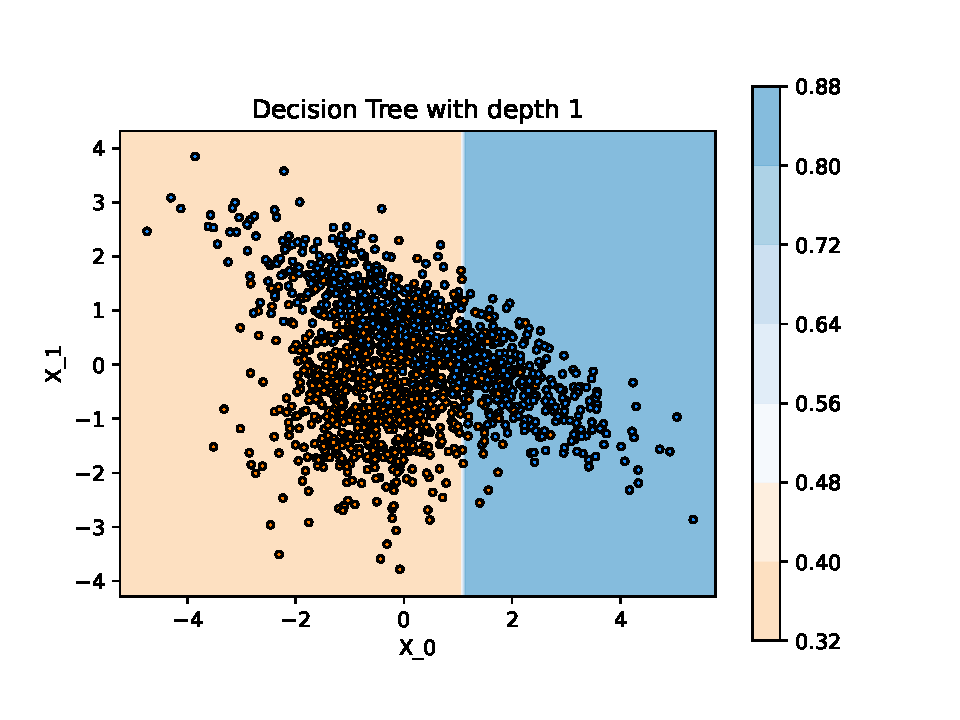
\includegraphics[width=.3\textwidth]{img/dt_1.pdf}\quad
		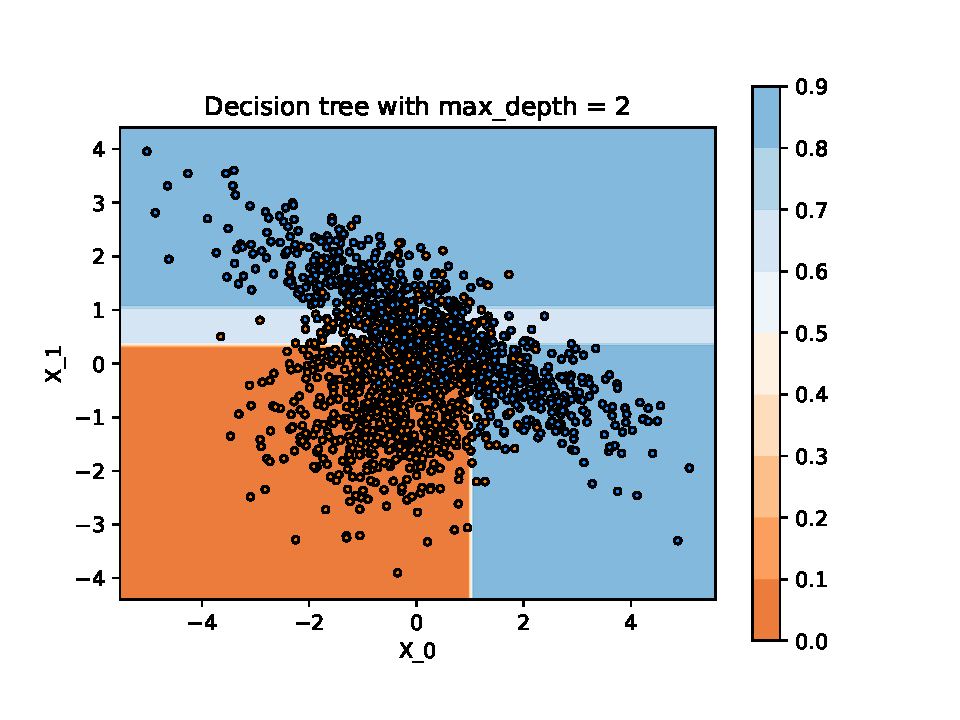
\includegraphics[width=.3\textwidth]{img/dt_2.pdf}\quad
		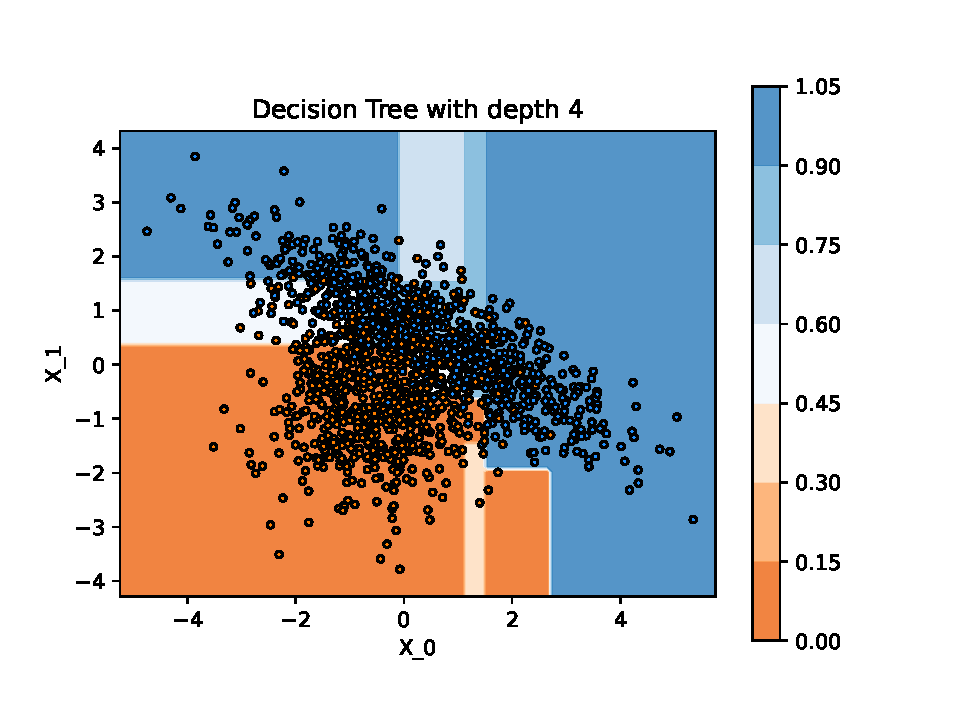
\includegraphics[width=.3\textwidth]{img/dt_4.pdf}
		
		\medskip
		
		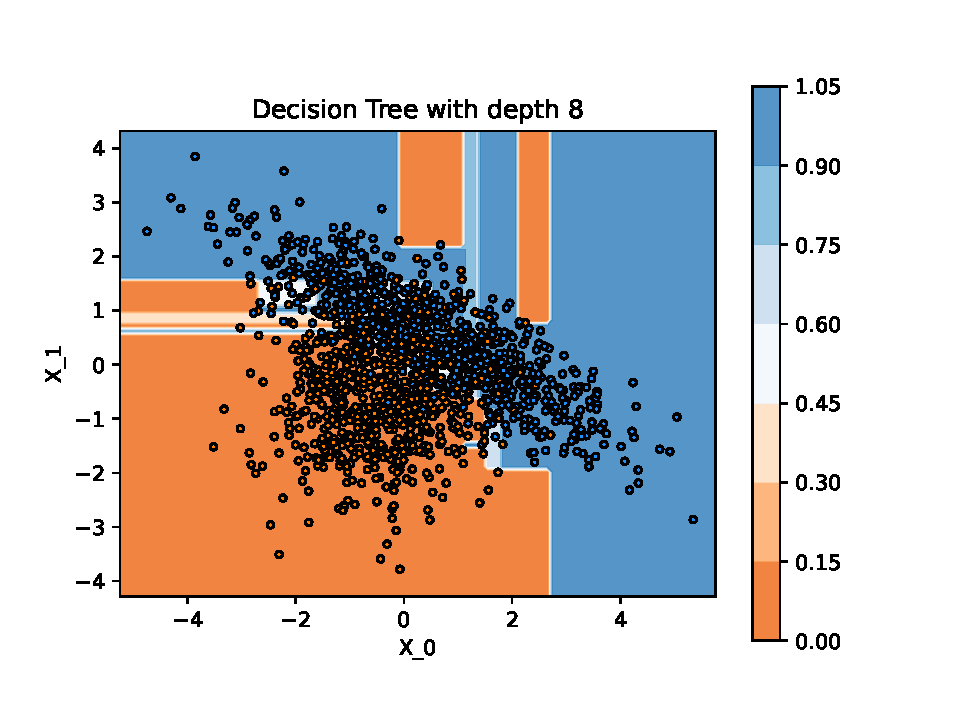
\includegraphics[width=.3\textwidth]{img/dt_8.pdf}\quad
		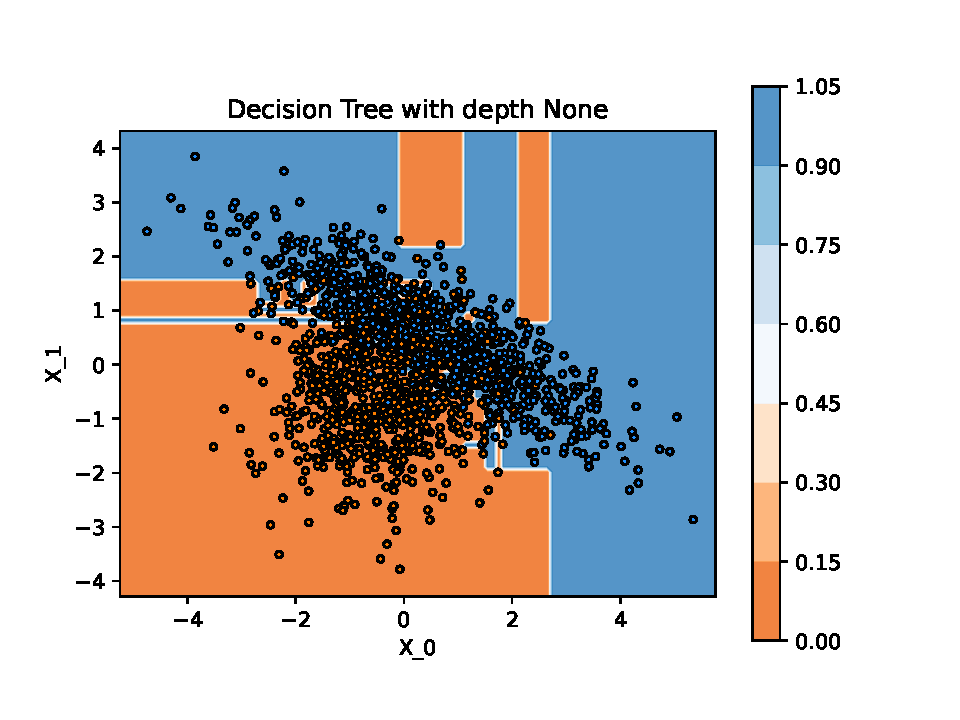
\includegraphics[width=.3\textwidth]{img/dt_None.pdf}
		
		\caption{Decision trees with different depths}
		\label{fig:dt}
		\end{figure}
	\item On one hand, when the depth is 1, the separation between areas is a simple line. 
	The model is too complex to be fit in this way so the depth 1 is clearly underfitting the problem. 
	For the depth 2, the model is more complex and fits the data better but it is still underfitting the problem.
	On the other hand, when the depth is 8, the model is too complex and the decision boundary is overfitting the problem. 
	When the hyperparameter \verb|depth| is set to \verb|None|, the nodes are expanded until all leaves are pure or until all leaves contain less than \verb|min_samples_split| samples, which is the minimum number of samples required to split an internal node.
	The best depth is 4 because it is the one that fits the problem the best. As demonstrated in the next point, the depth 4 is the one that gives the best accuracy.
	\item As previously said, when the depth becomes large, the model overfits the data, leading to a better confidence on the training set but a lower confidence on the test set.
\end{enumerate}

\subsection{Tests accuracy report}
	We report the results obtained for the different depths in the following table. The models were tested on 5 iterations of the dataset. 
	We can clearly see that the best depth is 4, as it gives the best accuracy while keeping the standard deviation low.
	When the depth gets past 4, the model overfits the data leading to decreased accuracy and increased standard deviation (the model is fitting the noise in the data).

	\begin{table}[H]
		\centering
		\begin{tabular}{|c|c|c|}
		\hline
		\verb|max_depth| & Mean & Standard Deviation \\ \hline
		1                                & 0.68 & 0.031              \\ \hline
		2                                & 0.80 & 0.021              \\ \hline
		4                                & 0.83 & 0.014              \\ \hline
		8                                & 0.81 & 0.016              \\ \hline
		None                             & 0.77 & 0.02               \\ \hline
		\end{tabular}
		\caption{Decision trees results}
		\label{tab:results-dt}
		\end{table}

	
	


\section{K-nearest neighbors}
	\subsection{Impact of the number of neighbors on the decision boundary}
	\begin{enumerate}[a)]
		\item This is the graphics with the 6 parameters.
		\begin{figure}[H]
			\centering
			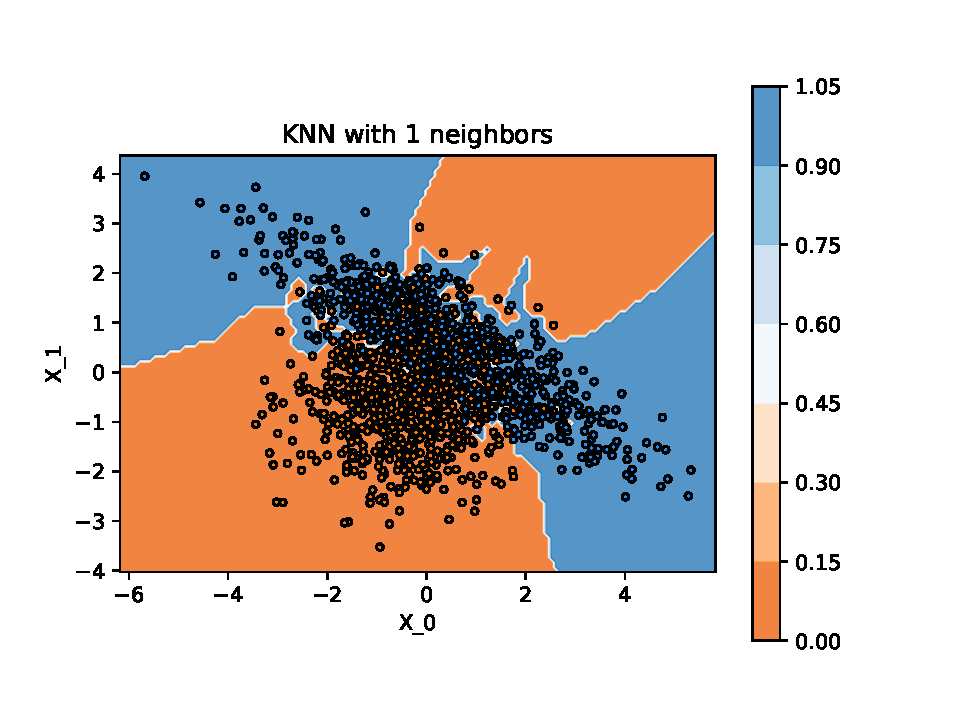
\includegraphics[width=.3\textwidth]{img/knn_1.pdf}\quad
			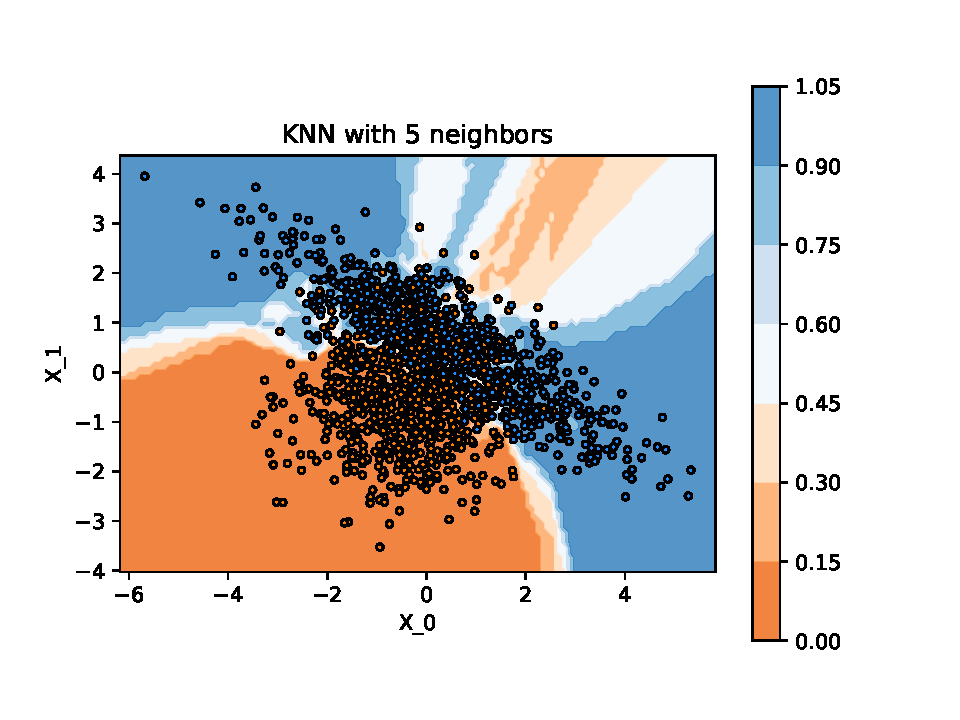
\includegraphics[width=.3\textwidth]{img/knn_5.pdf}\quad
			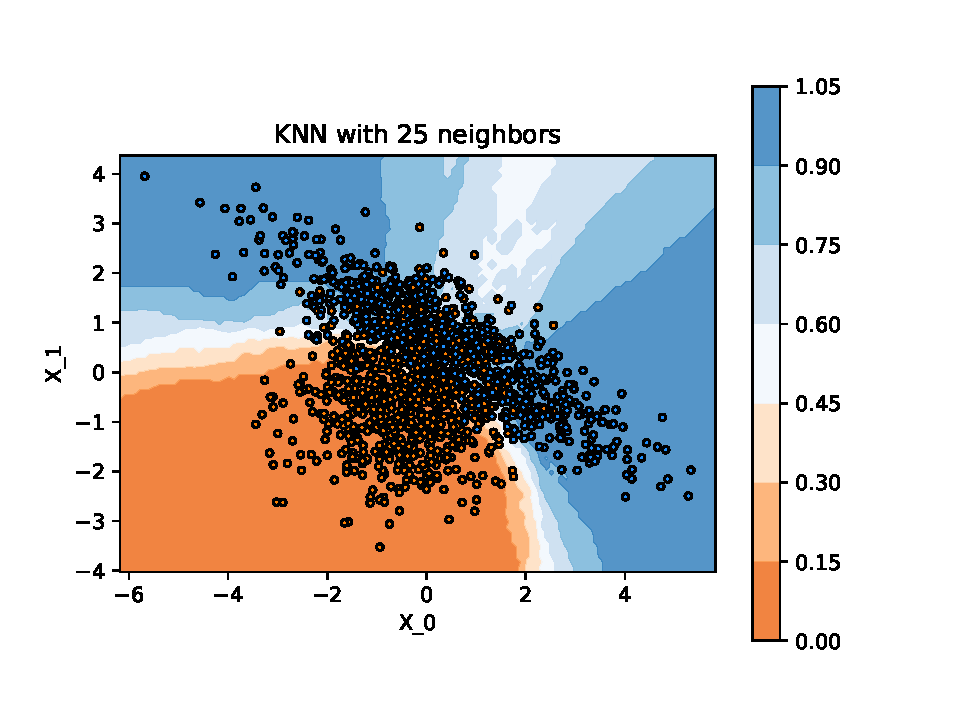
\includegraphics[width=.3\textwidth]{img/knn_25.pdf}\quad
			
			\medskip
			
			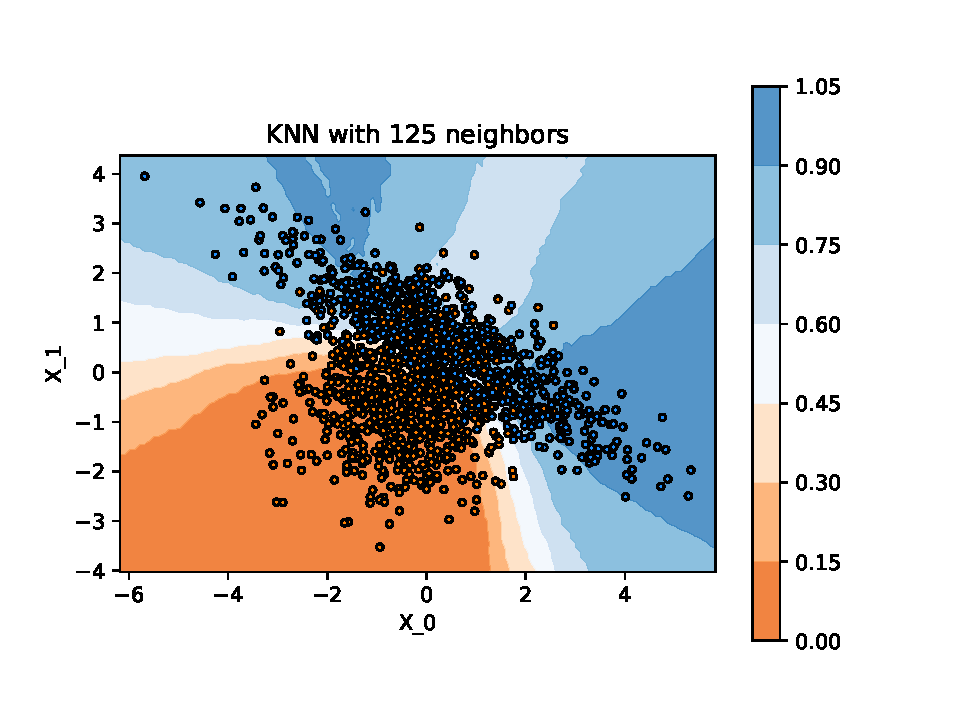
\includegraphics[width=.3\textwidth]{img/knn_125.pdf}\quad
			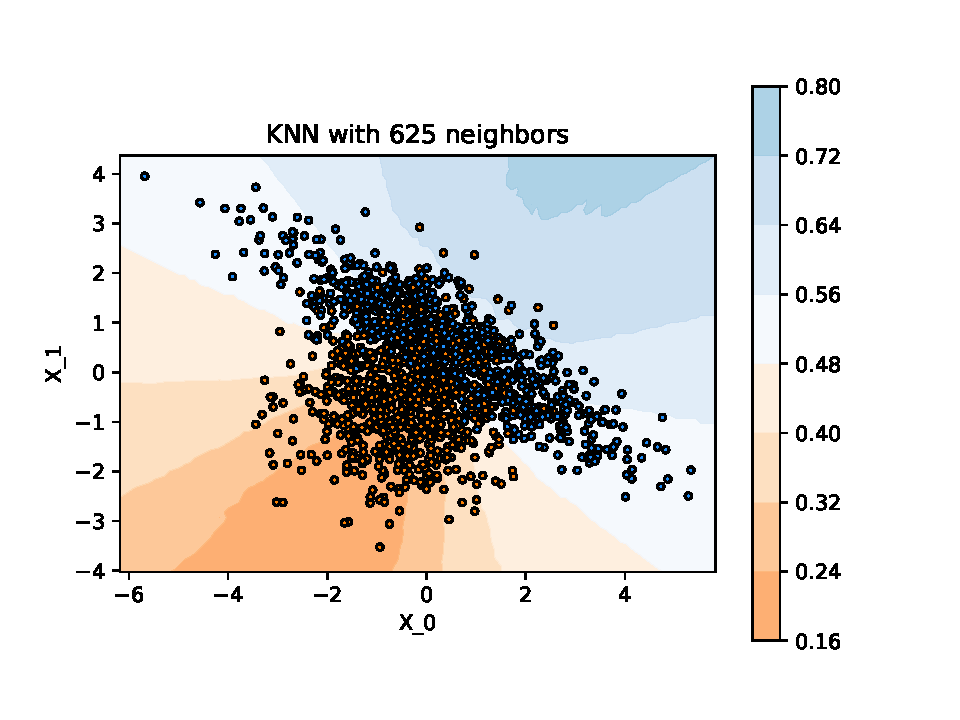
\includegraphics[width=.3\textwidth]{img/knn_625.pdf}\quad
			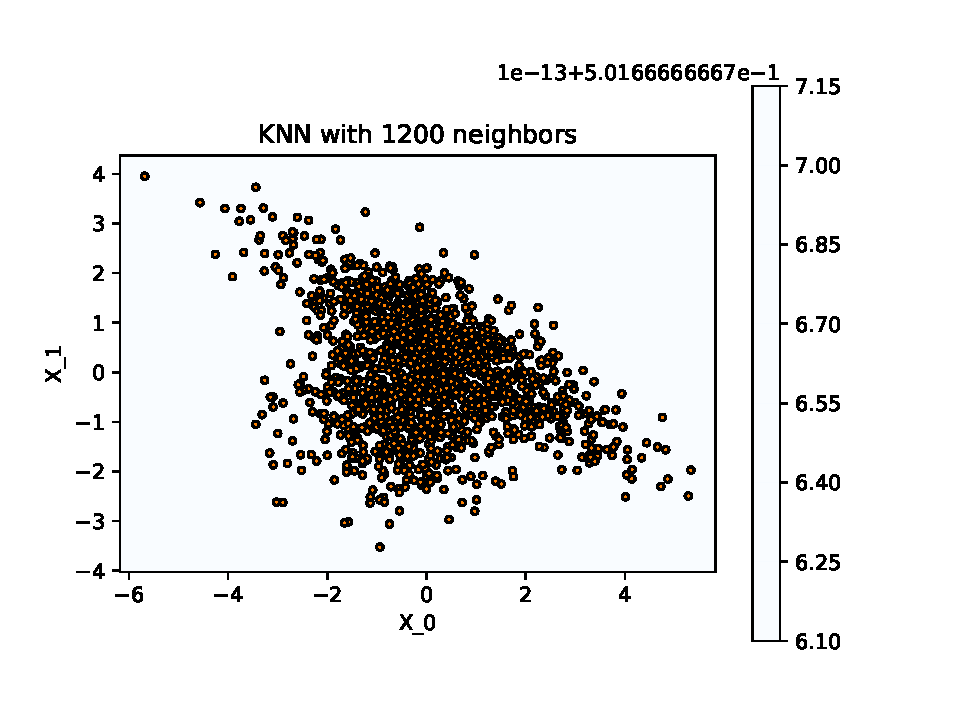
\includegraphics[width=.3\textwidth]{img/knn_1200.pdf}\quad
			
			\caption{K-nearest neighbors with different n\_neighbors values}
			\label{fig:knn}
		\end{figure}
		\item 
		The different boundaries are represented in figure 2. The lower the number of neighbors, the more the decision boundary is affected by the noise in the data (it starts to overfit). 
		When the number of neighbors increases, e.g for 5, 25 and 125, there's less overfitting and the decision boundary is more stable.
		When the number of neighbors gets even greater, e.g 625, the model starts to underfit the data, as it is not complex enough to fit the data.
		And in the worst case, when the number of neighbors is equal to the number of samples, the model simply makes the same prediction for every sample, which is the mean of the training set, giving the worst accuracy possible.
	\end{enumerate}
\subsection{Tests accuracy report}
Reporting to the table, we can see that the best number of neighbors is 125. 
Indeed, it gives good accuracy while keeping the standard deviation low. 
When the number of neighbors is too low, the model overfits the data and when it is too high, the model underfits the data.
	\begin{table}[H]
		\centering
		\begin{tabular}{|c|c|c|}
		\hline
		\verb|n_neighbors|               & Mean & Standard Deviation \\ \hline
		1                                & 0.78 & 0.024              \\ \hline
		5                                & 0.81 & 0.013              \\ \hline
		25                               & 0.84 & 0.013              \\ \hline
		125                              & 0.85 & 0.021              \\ \hline
		625                              & 0.81 & 0.010              \\ \hline
		1200                             & 0.48 & 0.014              \\ \hline

		\end{tabular}
		\caption{Decision trees results}
		\label{tab:results-knn}
	\end{table}



\section{Quadratic/Linear discriminant analysis}
\subsection{Decision boundaries}
In the 2 models, the decision boundaries is the curve where :
\begin{align}	
P(y=1|x) &= P(y=0|x)\\
\frac{f_0(x)\pi_0}{\sum^1_{l=0}f_l(x)\pi_l}&=\frac{f_1(x)\pi_1}{\sum^1_{l=0}f_l(x)\pi_l}\\
\end{align}
With : 
\begin{align}
	f_k(x) &= \frac{1}{2\pi\sqrt{|\Sigma_k|}}\exp\left(-\frac{1}{2}(x-\mu_k)^T\Sigma_k^{-1}(x-\mu_k)\right)
\end{align}
Dividing both sides by $P(y=1|x)$ and taking the logarithm, we get the following equation :
\begin{align}
	\log\frac{P(y=0|x)}{P(y=1|x)} = \log\frac{f_0(x)\pi_0}{f_1(x)\pi_1 }&=0\\
	\log\frac{f_0(x)}{f_1(x)} + \log\frac{\pi_0}{\pi_1}&= 0
\end{align}
The first term of the line 6 change between the Linear and Quadratic form. In the linear case, we have $|\Sigma_0|=|\Sigma_1|$ so in the division, we can simplify the 2 discriminant
and the quadratic form desappears. In the quadratic case, we have $|\Sigma_0|\neq|\Sigma_1|$ so we have to keep the quadratic form.\\
Linear case : 
\begin{align}
	\log\frac{\pi_0}{\pi_1} - \frac{1}{2}(\mu_0+\mu_1)^T\Sigma^{-1}(\mu_0-\mu_1) + x^T\Sigma^{-1}(\mu_0-\mu_1) = 0
\end{align}
Quadratic case : 
\begin{align}
	\log\frac{\pi_0}{\pi_1} - \frac{1}{2}(\mu_0+\mu_1)^T\Sigma^{-1}(\mu_0-\mu_1) + x^T\Sigma^{-1}(\mu_0-\mu_1) + \log\frac{|\Sigma_1|}{|\Sigma_0|} = 0
\end{align}
\subsection[]{Quadratic/Linear discriminant analysis}
As we can see, LDA is a special case of QDA where $\Sigma_0=\Sigma_1=\Sigma$. This is why the decision boundary is linear in LDA and quadratic in QDA.
It is also the reason why the curve of iso probbility is parallel line in LDA. We can also see that QDA is much more confident in general than LDA.

\begin{figure}[H]
	\centering
	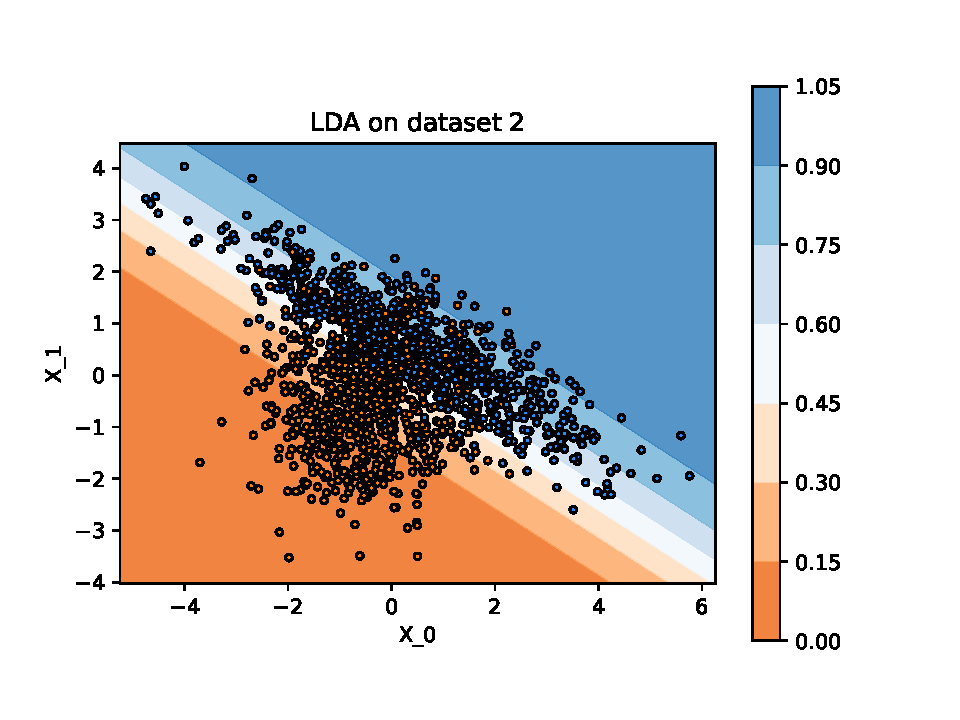
\includegraphics[width=.4\textwidth]{img/lda2.pdf}\quad
	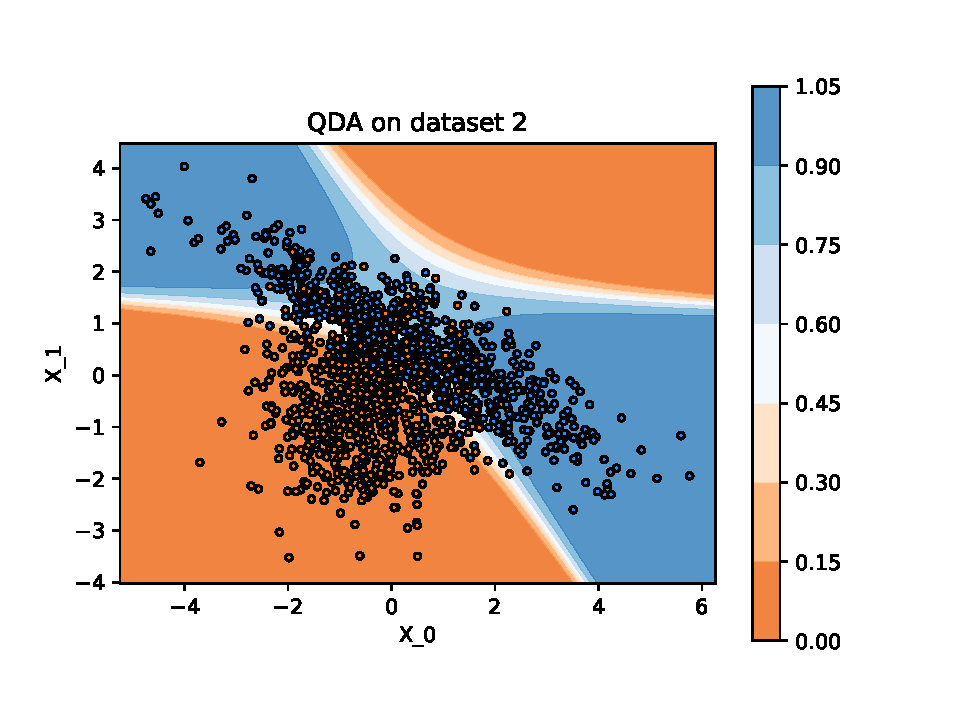
\includegraphics[width=.4\textwidth]{img/qda2.pdf}\quad
	
	\caption{Quadratic/Linear discriminant analysis}
	\label{fig:qdalda}
\end{figure}
\subsection{Tests accuracy report}
We can see that QDA is better than LDA in general. But the results are really close for dataset 1 because this dataset is created using circular gaussian distribution. 
So the covariance matrix is diagonal and the decision boundary is linear.
	\begin{table}[!h]
		\centering
		\begin{tabular}{|c|c|c|}
		\hline
		\verb|LDA QDA|                      & Mean & Standard Deviation \\ \hline
		LDA1                                & 0.85 & 0.068              \\ \hline
		QDA1                                & 0.86 & 0.057              \\ \hline
		LDA2                                & 0.72 & 0.053              \\ \hline
		QDA2                                & 0.76 & 0.062              \\ \hline
		\end{tabular}
		\caption{Decision trees results}
		\label{tab:results-qdalda}
	\end{table}


\section{Comparison}
\subsection{Tuning of hyperparameters}
	To tune our classifiers hyperparameters, we can use the cross-validation method.
	This method consists in splitting the dataset into $k$ folds.
	Then, we train the model on $k-1$ folds and test it on the remaining fold.
	We repeat this process $k$ times, each time using a different fold as the test set.
	Finally, we average the results to get the final accuracy. We used different values of the hyperparameters and we chose the one that gave the best accuracy.
	We implement this method in the \verb|tune.py| file using
	the \verb|GridSearchCV| class from the \verb|sklearn.model_selection| module. We used the 5-fold cross-validation method and the accuracy as the scoring parameter.
\subsection{Results of our implementation} 
	After finding the best hyperparameters, we trained the model using it and we tested it on 5 iterations of the dataset. Here are the results we obtained :
	\begin{table}[!h]
		\centering
		\begin{tabular}{|c|c|c|}
		\hline
								           & Mean & Standard Deviation \\ \hline
		KNN\_1\_tuned (neighbors = 25)       	& 0.91 & 0.012             \\ \hline
		DT\_1\_tuned (depth = 8)              & 0.89 & 0.018						  \\ \hline
		KNN\_2\_tuned (neighbors = 125)       & 0.83 & 0.019              \\ \hline
		DT\_2\_tuned (depth = 4)              & 0.82 & 0.02						  \\ \hline

		\end{tabular}
		\caption{Tuned hyperparameters results}
		\label{tab:results-tune}	
	\end{table}

\subsection{Comparison with the QDA/LDA results}

\end{document}